\section{Data preprocessing}
\label{sec:data-preprocessing}

From all predictors in Table \ref{table:predictors}, only SSRD, STRD, TSR, TP and TCC are used 
because they are the most relevant predictors. 
Since the Variables SSRD, STRD and TSR are all provided as accumulated fields, they first need to be decumulated.
This can be done by subtracting the value before the current value from the current value, for each day separately. 
Figure \ref{fig:strd-accumulated-vs-decumulated} shows both the accumulated and decumulated fields. 
A machine learning algorithm works better with the decumulated field since the decumulated field directly correlates 
with the power output of the solar plant.

\begin{figure}[h]%
    \centering
    \subfloat[\centering STRD accumulated]{{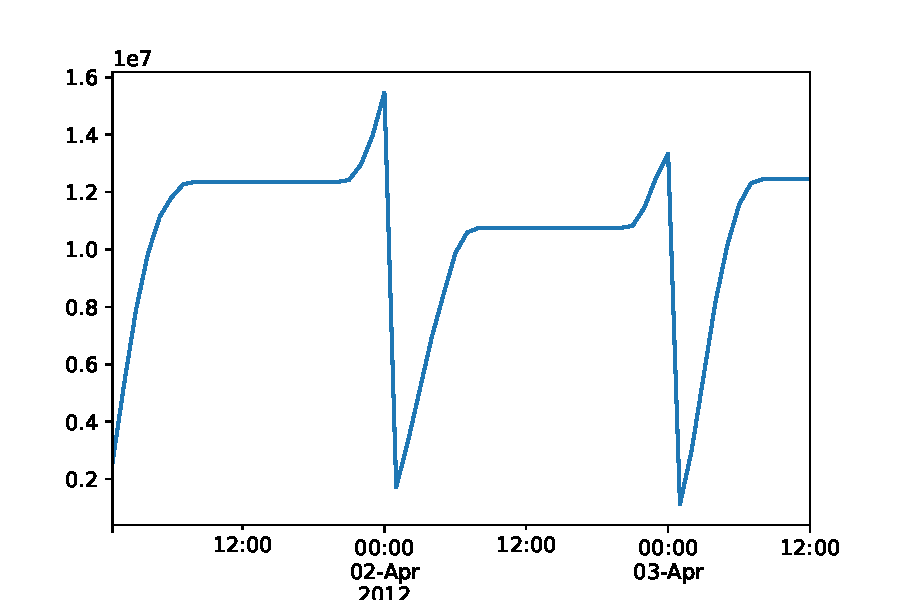
\includegraphics[width=7cm]{plots/strd_accumulated.pdf} }}%
    \qquad
    \subfloat[\centering STRD decumulated]{{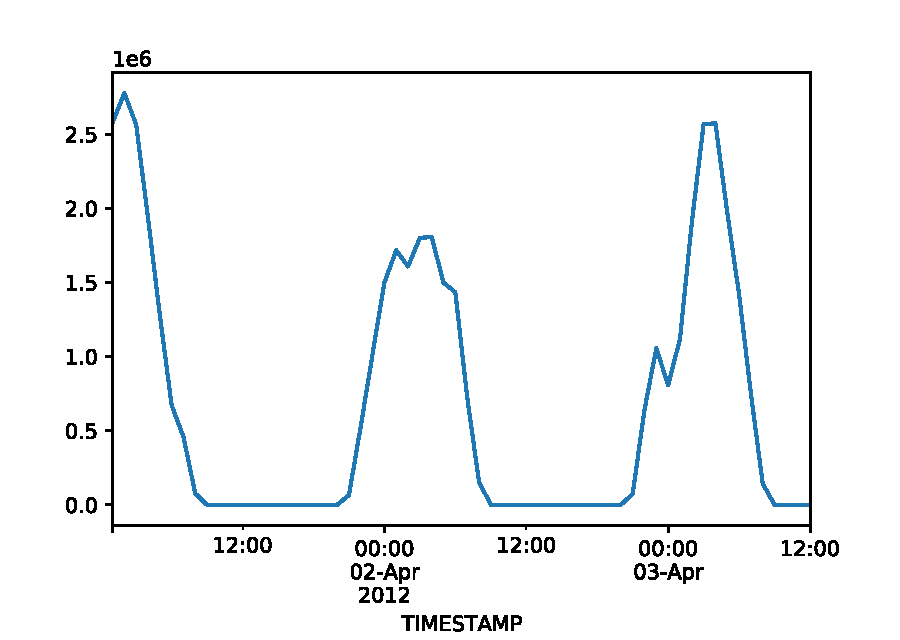
\includegraphics[width=7cm]{plots/strd_decumulated.pdf} }}%
    \caption[STRD accumulated vs. decumulated]{STRD accumulated vs. decumulated. 
    In order to get the actual data, we first need to subtract the previous point \(x_{t-1}\) from \(x_t\).}%
    \label{fig:strd-accumulated-vs-decumulated}%
\end{figure}